\section{Experiment}

This section describes the dataset, the prompting and sampling procedure used to generate LLM views, and the backtest protocol used to evaluate the BLM portfolios.

\subsection{Data Description}

We analyze daily adjusted prices from Yahoo Finance for a universe of the 50 largest S\&P 500 constituents as of March 26, 2025. The sample spans from June 2024 to June 2025. Simple daily returns are aggregated to $h$-day excess returns to match the rebalancing horizon. Note that because the universe is defined based on end‑of‑sample size ranks, results are conditional on this fixed universe and may reflect survivorship bias. 

We divide the sample into two non‑overlapping periods:
\begin{itemize}
    \item \textbf{Validation (June 1, 2024 -- August 31, 2024):} This 3-month period is used exclusively to tune the BLM hyperparameter $\tau$.
    \item \textbf{Test (September 1, 2024 -- June 30, 2025):} This 10-month period is reserved for out-of-sample evaluation. All model choices and parameters are fixed prior to this period.
\end{itemize}

We rebalance every ($h$=10) trading days. At each decision date $t$ (close), the LLM receives only information timestamped $\le$ $t$: the last $h$ trading days of prices and benchmark returns, plus static metadata (ticker, name, GICS sector/sub‑industry). The resulting views target the next $h$ trading days $[t+1, t+h]$. Portfolios are formed at $t+1$ open and held through $t+h$.
To quantify uncertainty, we perform $N=100$ independent inference runs per asset at each step. The resulting distribution of forecasts targets returns for the subsequent window $[t+1, t+h]$. Portfolios are formed at the open of $t+1$ and held until $t+h$.

\subsection{LLM Selection and Inference Protocol}

We elicit quantitative asset‑level forecasts from instruction‑tuned LLMs using a fixed schema prompt. 
To guarantee the validity of our out-of-sample evaluation, we selected models with training cutoffs pre-dating June 2024, which is well before the start of our backtesting. Table~\ref{tab:llm_summary} lists the specific versions, parameter sizes, release dates, and developers.

Inference uses vLLM \citep{kwon2023efficient} with fixed decoding settings to generate $N$ stochastic draws per asset per date.
The sample mean and variance form $(q_{i,t}, \Omega_{ii,t})$ as described in Section~\ref{sec:method}.
We employ the default sampling temperature of $T=1.0$. This choice is deliberate: rather than artificially collapsing the distribution via low-temperature greedy sampling, we aim to capture the model's intrinsic epistemic uncertainty. By sampling directly from the unscaled logit distribution, the resulting variance among the $N$ draws serves as a faithful proxy for the model's confidence ($\Omega$) in its view.

\begin{table}[h]
    \centering
    \begin{threeparttable}
        \caption{\textbf{Summary of LLMs used in this study.}}
        \label{tab:llm_summary}

        \small 
        
        \renewcommand{\arraystretch}{1.2}
        \begin{tabular}{llll}
            \hline
            \textbf{Model} & \textbf{Size} & \textbf{Release} & \textbf{Developer} \\
            \hline
            \textbf{\texttt{Gemma-7B}} \cite{team2024gemma}       & 7B      & Feb 2024 & Google DeepMind \\
            \textbf{\texttt{Qwen-2-7B}} \cite{yang2024qwen2technicalreport}    & 7B      & Jun 2024 & Alibaba Cloud \\
            \textbf{\texttt{Llama-3.1-8B}} \cite{dubey2024llama}   & 8B      & Jul 2024 & Meta \\
            \textbf{\texttt{GPT-4o-mini}} \cite{openai2024gpt4o}    & 8B \tnote{a} & Jul 2024 & OpenAI \\
            \hline
        \end{tabular}
        \begin{tablenotes}
            \scriptsize
            \item[a] Although the exact size of \texttt{GPT-4o-mini} has not been officially disclosed, \cite{abacha2024medec} estimate it to be within the 8 billion parameter range, making it comparable to the open-source models used in our study.
        \end{tablenotes}
    \end{threeparttable}
\end{table}














\section{Analysis}

We conduct an empirical backtest to evaluate the performance of our proposed framework, which integrates LLM-generated views into the BLM. To structure our analysis, we address the following key research questions:

\begin{itemize}
    \item[\textbf{RQ1}] \textit{(Performance \& Accuracy)} How does the LLM-BLM framework compare to traditional benchmarks (EW, MVO) in terms of risk-adjusted portfolio returns, and how accurate are the underlying asset price forecasts generated by each LLM?
    \item[\textbf{RQ2}] \textit{(Style: View)} Do different LLMs exhibit distinct and characterizable investment styles in their predictive view distributions, and if so, how do they differ in terms of bias, dispersion, and conviction?
    \item[\textbf{RQ3}] \textit{(Style: Confidence)} What is the relationship between the confidence of the LLM-generated predictions and their realized prediction accuracy?
\end{itemize}

The subsequent sections are structured to answer each of these questions in turn. Our evaluation follows a two-stage process: first, we optimize the model's key hyperparameter, $\tau$, which was introduced in Equation~\ref{eq:BlackLitterman}. Second, we assess the final portfolio performance on an unseen test period to address our research questions.

\subsection{Experimental Setup}
We evaluate four BLM portfolios such as \textbf{\texttt{BLM‑Gemma}}, \textbf{\texttt{BLM‑Qwen}}, \textbf{\texttt{BLM‑Llama}}, and \textbf{\texttt{BLM‑GPT}} against three benchmarks: (i) Market (S\&P 500 total‑return index), (ii) EW (equal‑weight, long‑only), and (iii) MVO (mean–variance using the same $h$-horizon covariance and long‑only constraints). We report annualized geometric return; annualized volatility (daily standard deviation multiplied by $\sqrt{252}$; Sharpe relative to the 3‑month Treasury bill (interpolated to daily); maximum drawdown from daily equity; and 95\% historical one‑day VaR and CVaR. All metrics are computed from net daily returns. Transaction costs are applied as $c\sum_i |w_{i,t}-w_{i,t^-}|$ at each rebalance with $c=10$ bps per one‑way trade.

\textbf{Hyperparameter tuning.} We focus on tuning the scalar $\tau$, which scales the prior uncertainty in the BLM update. We set the initial value $\tau_{\text{init}}$ based on the ratio of view uncertainty to asset covariance over the validation period $T_{\text{val}}$:
\begin{equation}
\tau_{\text{init}}=\frac{1}{|T_{\text{val}}|}\sum_{t\in T_{\text{val}}}\frac{\bar{\Omega}_t}{\bar{\Sigma}_t},    
\end{equation}
where $\bar{\Omega}_t$ and $\bar{\Sigma}_t$ denote the average of the diagonal elements of $\mathbf{\Omega}_t$ and the elements of $\boldsymbol{\Sigma}_t$, respectively. We then perform a centered grid search over $\{0.5,0.75,1,1.25,1.5\}\times\tau_{\text{init}}$ and select the optimal $\tau^\star$ separately for each LLM, holding it fixed during the test evaluation.

\subsection{RQ1: Portfolio Performance \& Accuracy}
Table~\ref{tab:vertical_performance_comparison} and Figure~\ref{fig:cumulative_returns} summarize the comparative performance analysis of four proposed BLM-based models against two traditional benchmarks: the EW and MVO portfolios. The evaluation encompasses various metrics, including absolute returns, risk-adjusted returns, and downside risk.
The analysis reveals a strong performance from the BLM-based models, particularly \textbf{\texttt{BLM-Qwen}} and \textbf{\texttt{BLM-Llama}}. \textbf{\texttt{BLM-Qwen}} achieved the highest CAGR of 0.2811, closely followed by \textbf{\texttt{BLM-Llama}} at 0.2751. Both significantly outperformed the traditional benchmarks, EW (0.1907) and MVO (0.0607). In terms of risk-adjusted returns, measured by the annualized Sharpe Ratio, Sharpe (ann.), \textbf{\texttt{BLM-Llama}} delivered the top performance with a ratio of 1.2286. \textbf{\texttt{BLM-Qwen}} secured the second-highest position at 1.0624. This indicates that both models generated superior excess returns per unit of risk, far exceeding the benchmarks EW (0.8937) and MVO (0.2793).

\begin{table}[H]
% 문서 상단(preamble)에 다음 두 줄을 추가하세요.
% \usepackage{siunitx}
% \usepackage{soul} % \ul (밑줄) 명령을 위해

% \begin{table*}[t!]
    \centering
    \renewcommand{\arraystretch}{1.2}
    % siunitx 설정: 숫자를 소수점 4자리로 반올림하고, 굵은 글씨체를 감지하도록 설정
    \sisetup{
        round-mode=places,
        round-precision=4,
        detect-weight=true,
        table-format=-1.4
    }
    % 글자 크기를 약간 줄이고, 열 사이의 간격을 조절하여 공간을 확보합니다
    \footnotesize % \small \footnotesize 
    \setlength{\tabcolsep}{2.8pt} % 기본값(6pt)보다 간격을 줄입니다.
    \begin{tabularx}{\columnwidth}{ % 전체 너비를 현재 열 너비(\columnwidth)에 맞춥니다.
        >{\RaggedRight}X  % 첫 번째 열을 유연한 X타입으로 변경해 자동 줄바꿈을 적용합니다.
        S[table-format=1.4]
        S[table-format=1.4]
        S[table-format=-1.4]
        S[table-format=1.4]
        S[table-format=1.4]
        S[table-format=-1.4]
    }
        \hline
        {Metric} & {EW} & {MVO} & {\textbf{\texttt{BLM-Gemma}}} & {\textbf{\texttt{BLM-Qwen}}} & {\textbf{\texttt{BLM-Llama}}} & {\textbf{\texttt{BLM-GPT}}} \\
        \hline
        CAGR \(\uparrow\) & 0.1907 & 0.0607 & 0.1590 & \bfseries 0.2811 & \ul{0.2751} & 0.0768 \\
        mean \(\uparrow\) & 0.0008 & 0.0004 & 0.0007 & \bfseries 0.0011 & \ul{0.0010} & 0.0004 \\
        std \(\downarrow\) & \bfseries 0.0122 & 0.0179 & 0.0156 & 0.0152 & \ul{0.0124} & 0.0132 \\
        Sharpe \(\uparrow\) & 0.0563 & 0.0176 & 0.0402 & \ul{0.0669} & \bfseries 0.0774 & 0.0228 \\
        mean (ann.) \(\uparrow\) & 0.1932 & 0.0994 & 0.1784 & \bfseries 0.2763 & \ul{0.2627} & 0.0958 \\
        std (ann.) \(\downarrow\) & \bfseries 0.1938 & 0.2841 & 0.2481 & 0.2413 & \ul{0.1975} & 0.2093 \\
        Sharpe (ann.) \(\uparrow\) & 0.8937 & 0.2793 & 0.6386 & \ul{1.0624} & \bfseries 1.2286 & 0.3619 \\
        MDD \(\uparrow\) & -0.1688 & -0.1620 & -0.1551 & \bfseries -0.1375 & \ul{-0.1383} & -0.1649 \\
        VaR95\% \(\uparrow\) & -0.0171 & -0.0259 & \ul{-0.0168} & -0.0182 & -0.0169 & \bfseries -0.0157 \\
        CVaR95\% \(\uparrow\) & \bfseries -0.0280 & -0.0448 & -0.0372 & -0.0320 & \ul{-0.0283} & -0.0312 \\
        % MSE $\downarrow$ & 0 & 0.9376 & 1.2373 & \bfseries 0.5125 & \ul{0.5288} & 0.6505 \\
        % RMSE $\downarrow$ & 0 & 0.9683 & 1.1123 & \bfseries 0.7159 & \ul{0.7272} & 0.8066 \\
        % MAE $\downarrow$ & 0 & 0.6989 & 0.8608 & \bfseries 0.5168 & \ul{0.5281} & 0.5702 \\
        \hline
    \end{tabularx}
    \caption{
    \textbf{Out-of-sample Investment Performance of Portfolios}
    % Comparative Analysis of Out-of-sample Quantitative Performance and Risk Metrics for All Portfolios. BLM-Qwen achieved the highest absolute return (CAGR of 0.2811), while BLM-Llama delivered the best risk-adjusted return (Sharpe (ann.) of 1.2286). Both strategies significantly surpassed the baseline, demonstrating the framework's ability to generate consistent alpha.
    }
    \label{tab:vertical_performance_comparison}
% \end{table*}
 % \label{tab:vertical_performance_comparison}
\end{table}
Regarding volatility, std (ann.), the EW portfolio was the most stable with a value of 0.1938, underscoring the benefits of simple diversification. However, \textbf{\texttt{BLM-Llama}} was a very close second with a volatility of 0.1975, indicating effective risk management. In downside risk, the BLM models also excelled. \textbf{\texttt{BLM-Qwen}} posted the lowest MDD at -0.1375, with \textbf{\texttt{BLM-Llama}} following closely at -0.1383, both demonstrating significantly better capital preservation than the benchmarks during downturns.
The other LLM-based strategies showed mixed results. The \textbf{\texttt{BLM-Gemma}} model delivered a modest positive CAGR of 0.1590, while the \textbf{\texttt{BLM-GPT}} model lagged with a CAGR of 0.0768, performing similarly to the MVO benchmark in terms of returns.

Notably, the hierarchy of investment performance mirrors the hierarchy of predictive accuracy shown in Table~\ref{tab:prediction_metrics}. In this analysis, predictive accuracy is measured by regression metrics (MSE, RMSE, and MAE) of the return forecasts and classification metrics (accuracy, precision, recall, and F1-score) derived from the confusion matrix of directional (up/down) movements.
\textbf{\texttt{BLM-Qwen}} and \textbf{\texttt{BLM-Llama}}, which secured the top investment rankings, exhibited the lowest regression errors and superior classification scores. This suggests that the generated views provided highly accurate directional signals, which the BLM framework successfully translated into profitable allocation decisions.
\begin{figure}[H]
    \centering
    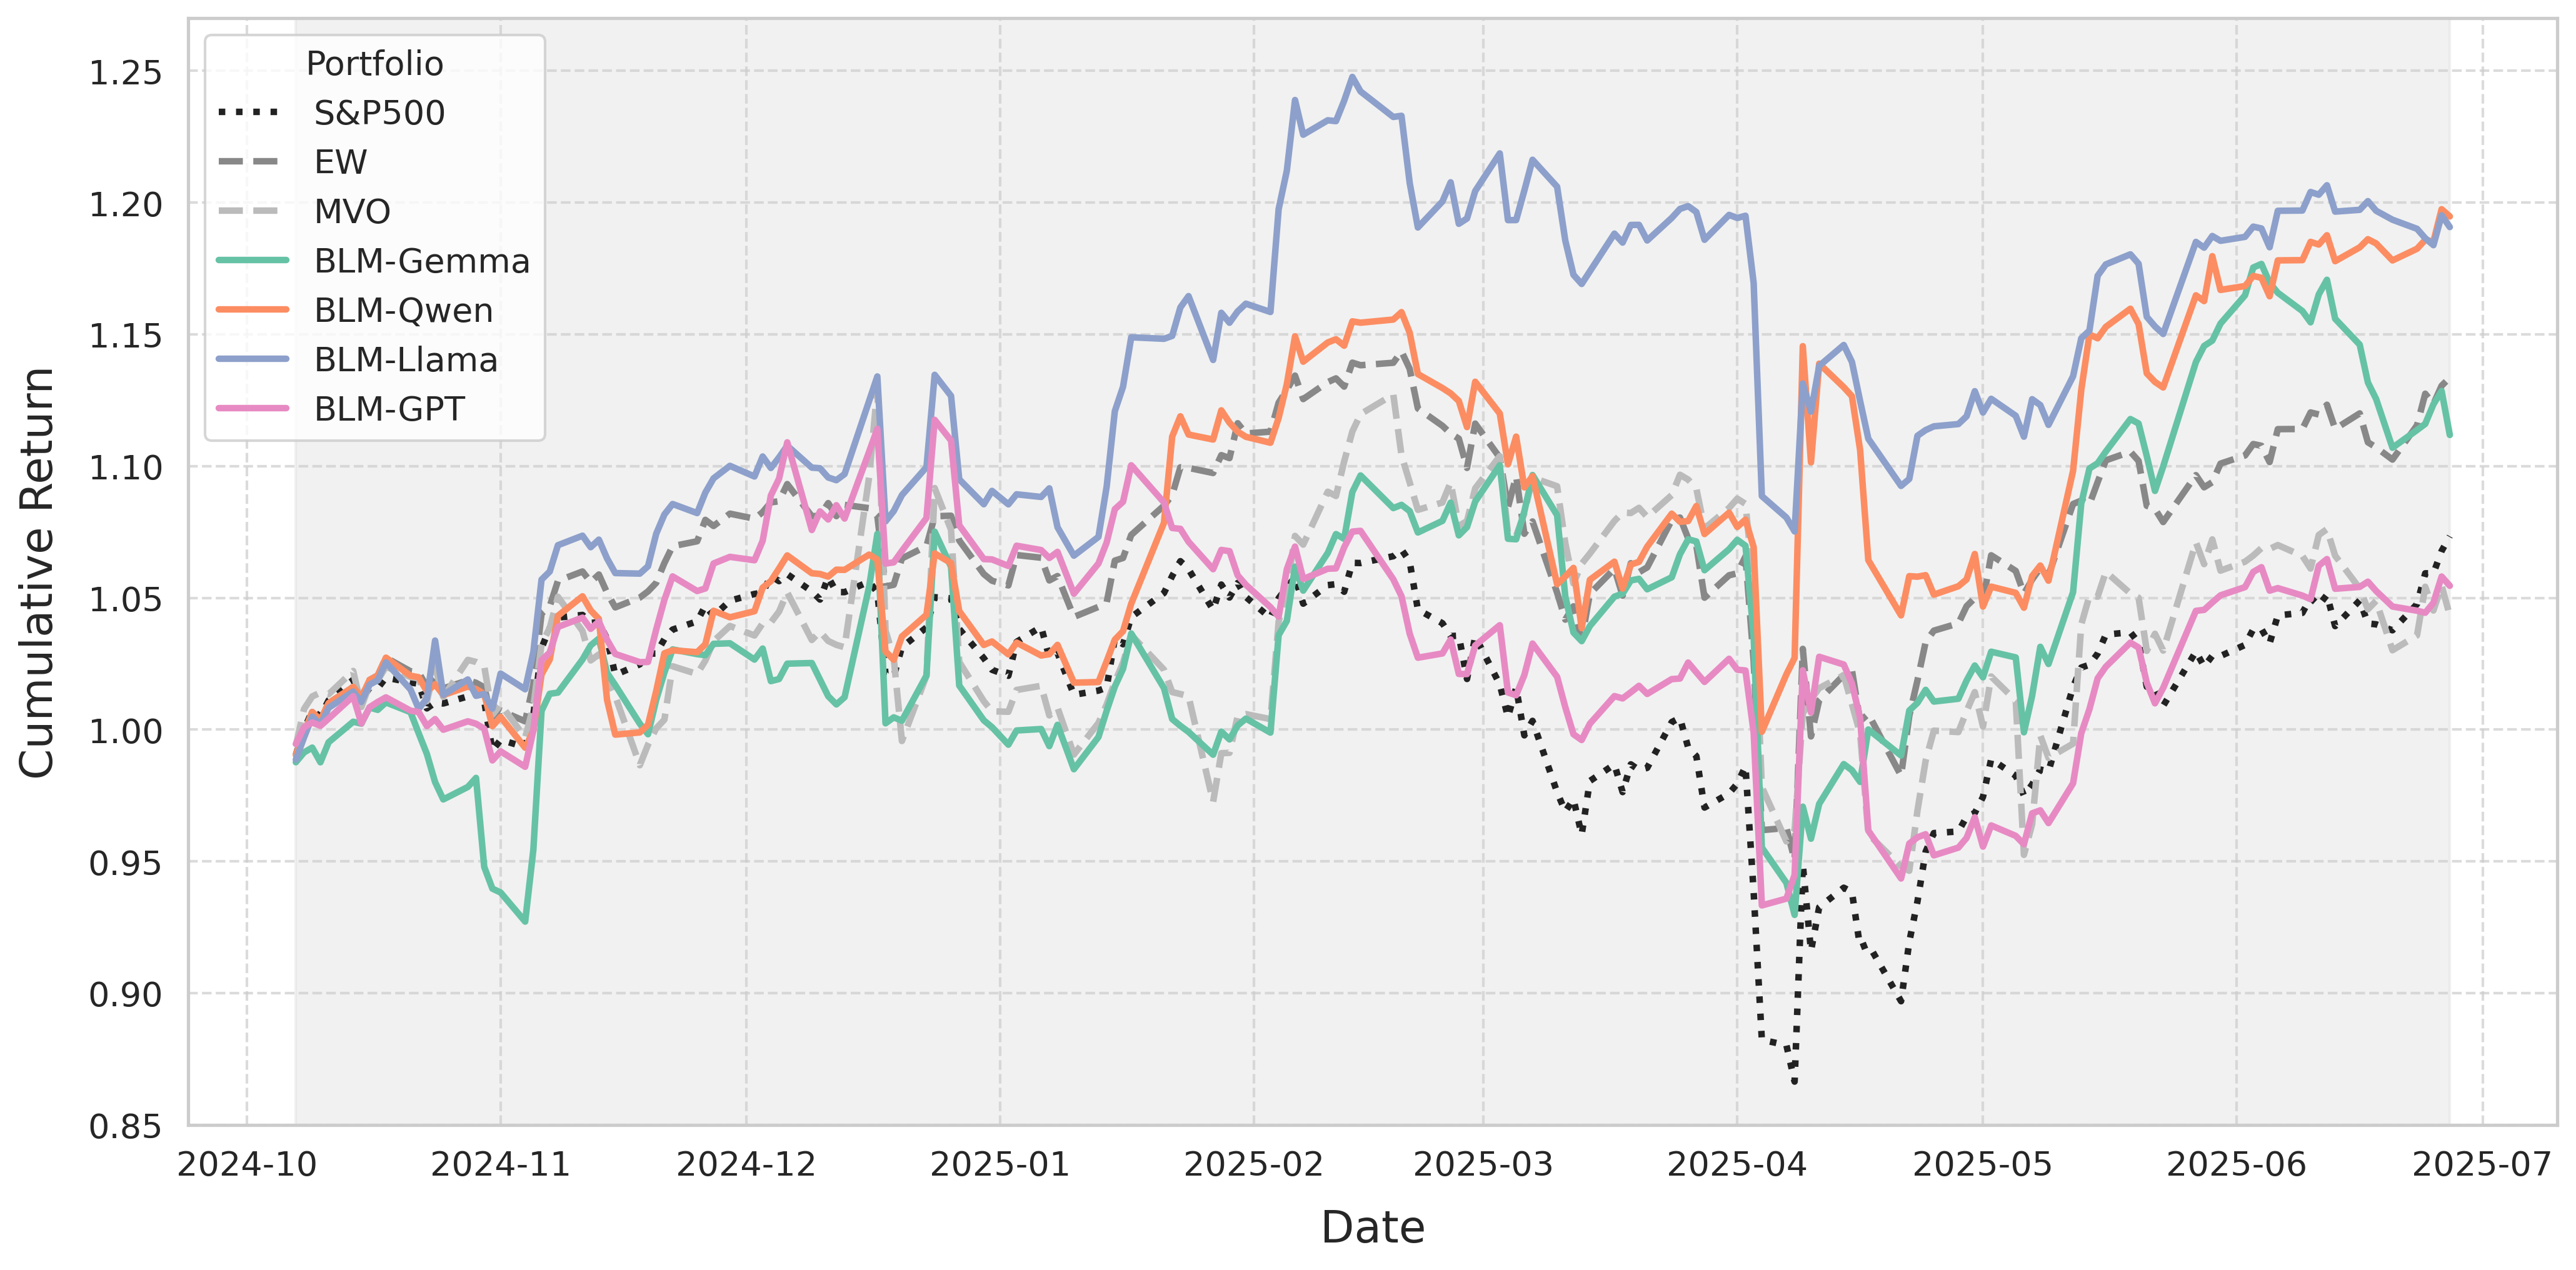
\includegraphics[width=0.9\textwidth]{figure/cumulative_returns_prompt4.png}  
    \caption{
    \textbf{Comparative Analysis of Cumulative Returns for BLM and Benchmark Portfolios.} The results highlight the significant outperformance of the \textbf{\texttt{BLM-Qwen}} and \textbf{\texttt{BLM-Llama}} strategies, which consistently generated higher returns compared to both the market index and conventional quantitative models.}
    \label{fig:cumulative_returns}  
\end{figure}
Conversely, the underperformance of \textbf{\texttt{BLM-Gemma}} and \textbf{\texttt{BLM-GPT}} corresponds to their higher prediction errors. High regression errors and lower classification accuracy in these models likely introduced noise into the posterior estimates, degrading the efficiency of the optimized portfolios.


% \begin{table}[h!]
%     \centering
%     \caption{\textbf{Comparison of Prediction Errors and Classification Metrics}}
%     \label{tab:prediction_metrics}
%     \renewcommand{\arraystretch}{1.2}
%     % siunitx 설정: 숫자를 소수점 4자리로 정렬
%     \sisetup{
%         round-mode=places,
%         round-precision=4,
%         detect-weight=true,
%         table-format=1.4 % 정수 1자리, 소수 4자리
%     }
%     \small
%     \setlength{\tabcolsep}{5pt}
%     % tabularx 대신 tabular와 siunitx의 S column을 사용
%     \begin{tabular}{l S S S S S}
%     \toprule
%     \textbf{Metric} & {\textbf{MVO}} & {\textbf{\texttt{BLM-Gemma}}} & {\textbf{\texttt{BLM-Qwen}}} & {\textbf{\texttt{BLM-Llama}}} & {\textbf{\texttt{BLM-GPT}}} \\
%     \midrule
%     CAGR \(\uparrow\) & 0.0607 & 0.1590 & \bfseries 0.2811 & \ul{0.2751} & 0.0768 \\
%     Sharpe \(\uparrow\) & 0.0176 & 0.0402 & \ul{0.0669} & \bfseries 0.0774 & 0.0228 \\
%     \midrule
%     MSE $\downarrow$  & 0.9376 & 1.2373 & \bfseries 0.5125 & \ul{0.5288} & 0.6505 \\
%     RMSE $\downarrow$ & 0.9683 & 1.1123 & \bfseries 0.7159 & \ul{0.7272} & 0.8066 \\
%     MAE $\downarrow$  & 0.6989 & 0.8608 & \bfseries 0.5168 & \ul{0.5281} & 0.5702 \\
%     \midrule
%     Accuracy $\uparrow$  & {0.5059} & 0.4719 & \bfseries 0.5719 & \ul{0.5437} & 0.5215 \\
%     Precision $\uparrow$ & {0.5689} & 0.5648 & \bfseries 0.5781 & \ul{0.5689} & 0.5645 \\
%     Recall $\uparrow$    & {0.5711} & 0.3437 & \bfseries 0.9367 & \ul{0.8424} & 0.7235 \\
%     F1 $\uparrow$        & {0.5700} & 0.4273 & \bfseries 0.7150 & \ul{0.6792} & 0.6342 \\
%     \bottomrule
%     \end{tabular}
% \end{table}


\begin{table}[h!]
    \centering
    \caption{\textbf{Comparison of Portfolio and Predictive Performance Metrics}}
    \label{tab:prediction_metrics}
    \renewcommand{\arraystretch}{1.2}
    
    % siunitx 설정
    \sisetup{
        round-mode=places,
        round-precision=4,
        detect-weight=true,
        table-format=1.4
    }
    \small
    \setlength{\tabcolsep}{4pt} % 컬럼이 늘어났으므로 간격을 조금 좁힘
    
    % 컬럼 정의: 맨 앞에 그룹용 'l' 추가 (총 7개 컬럼)
    \begin{tabular}{l l S S S S S}
    \toprule
    & \textbf{Metric} & {\textbf{MVO}} & {\textbf{\texttt{BLM-Gemma}}} & {\textbf{\texttt{BLM-Qwen}}} & {\textbf{\texttt{BLM-Llama}}} & {\textbf{\texttt{BLM-GPT}}} \\
    \midrule
    
    % --- Group 1: Portfolio Performance ---
    \multirow{2}{*}{\shortstack[l]{\textbf{Portfolio}\\\textbf{Performance}}} 
        & CAGR \(\uparrow\)    & 0.0607 & 0.1590 & \bfseries 0.2811 & \ul{0.2751} & 0.0768 \\
        & Sharpe \(\uparrow\)  & 0.0176 & 0.0402 & \ul{0.0669} & \bfseries 0.0774 & 0.0228 \\
    \midrule
    
    % --- Group 2: Regression ---
    \multirow{3}{*}{\shortstack[l]{\textbf{Predictive}\\\textbf{Performance}\\\textbf{(Regression)}}} 
        & MSE $\downarrow$     & 0.9376 & 1.2373 & \bfseries 0.5125 & \ul{0.5288} & 0.6505 \\
        & RMSE $\downarrow$    & 0.9683 & 1.1123 & \bfseries 0.7159 & \ul{0.7272} & 0.8066 \\
        & MAE $\downarrow$     & 0.6989 & 0.8608 & \bfseries 0.5168 & \ul{0.5281} & 0.5702 \\
    \midrule
    
    % --- Group 3: Classification ---
    \multirow{4}{*}{\shortstack[l]{\textbf{Predictive}\\\textbf{Performance}\\\textbf{(Classification)}}} 
        & Accuracy $\uparrow$  & {0.5059} & 0.4719 & \bfseries 0.5719 & \ul{0.5437} & 0.5215 \\
        & Precision $\uparrow$ & {0.5689} & 0.5648 & \bfseries 0.5781 & \ul{0.5689} & 0.5645 \\
        & Recall $\uparrow$    & {0.5711} & 0.3437 & \bfseries 0.9367 & \ul{0.8424} & 0.7235 \\
        & F1 $\uparrow$        & {0.5700} & 0.4273 & \bfseries 0.7150 & \ul{0.6792} & 0.6342 \\
    \bottomrule
    \end{tabular}
\end{table}
 % \label{tab:prediction_errors}



\subsection{RQ2: Investment Styles - View}

To further investigate the characteristics of the formulated asset views, we analyzed the distribution of their values. Figure~\ref{fig:boxplot} displays a time-series of these distributions. Since a single view corresponds to a specific asset, each boxplot on the chart represents the cross-sectional distribution of views across the $n$ assets for that rebalancing period. This visualization reveals how the dispersion of the model's expected returns evolves over time. The y-axis is clipped to a range of -0.03 to 0.03 for clarity, and the summary statistics in Table~\ref{tab:view_statistics} provide details on the aggregate distribution across all periods.

\begin{figure}[H]
    \centering
    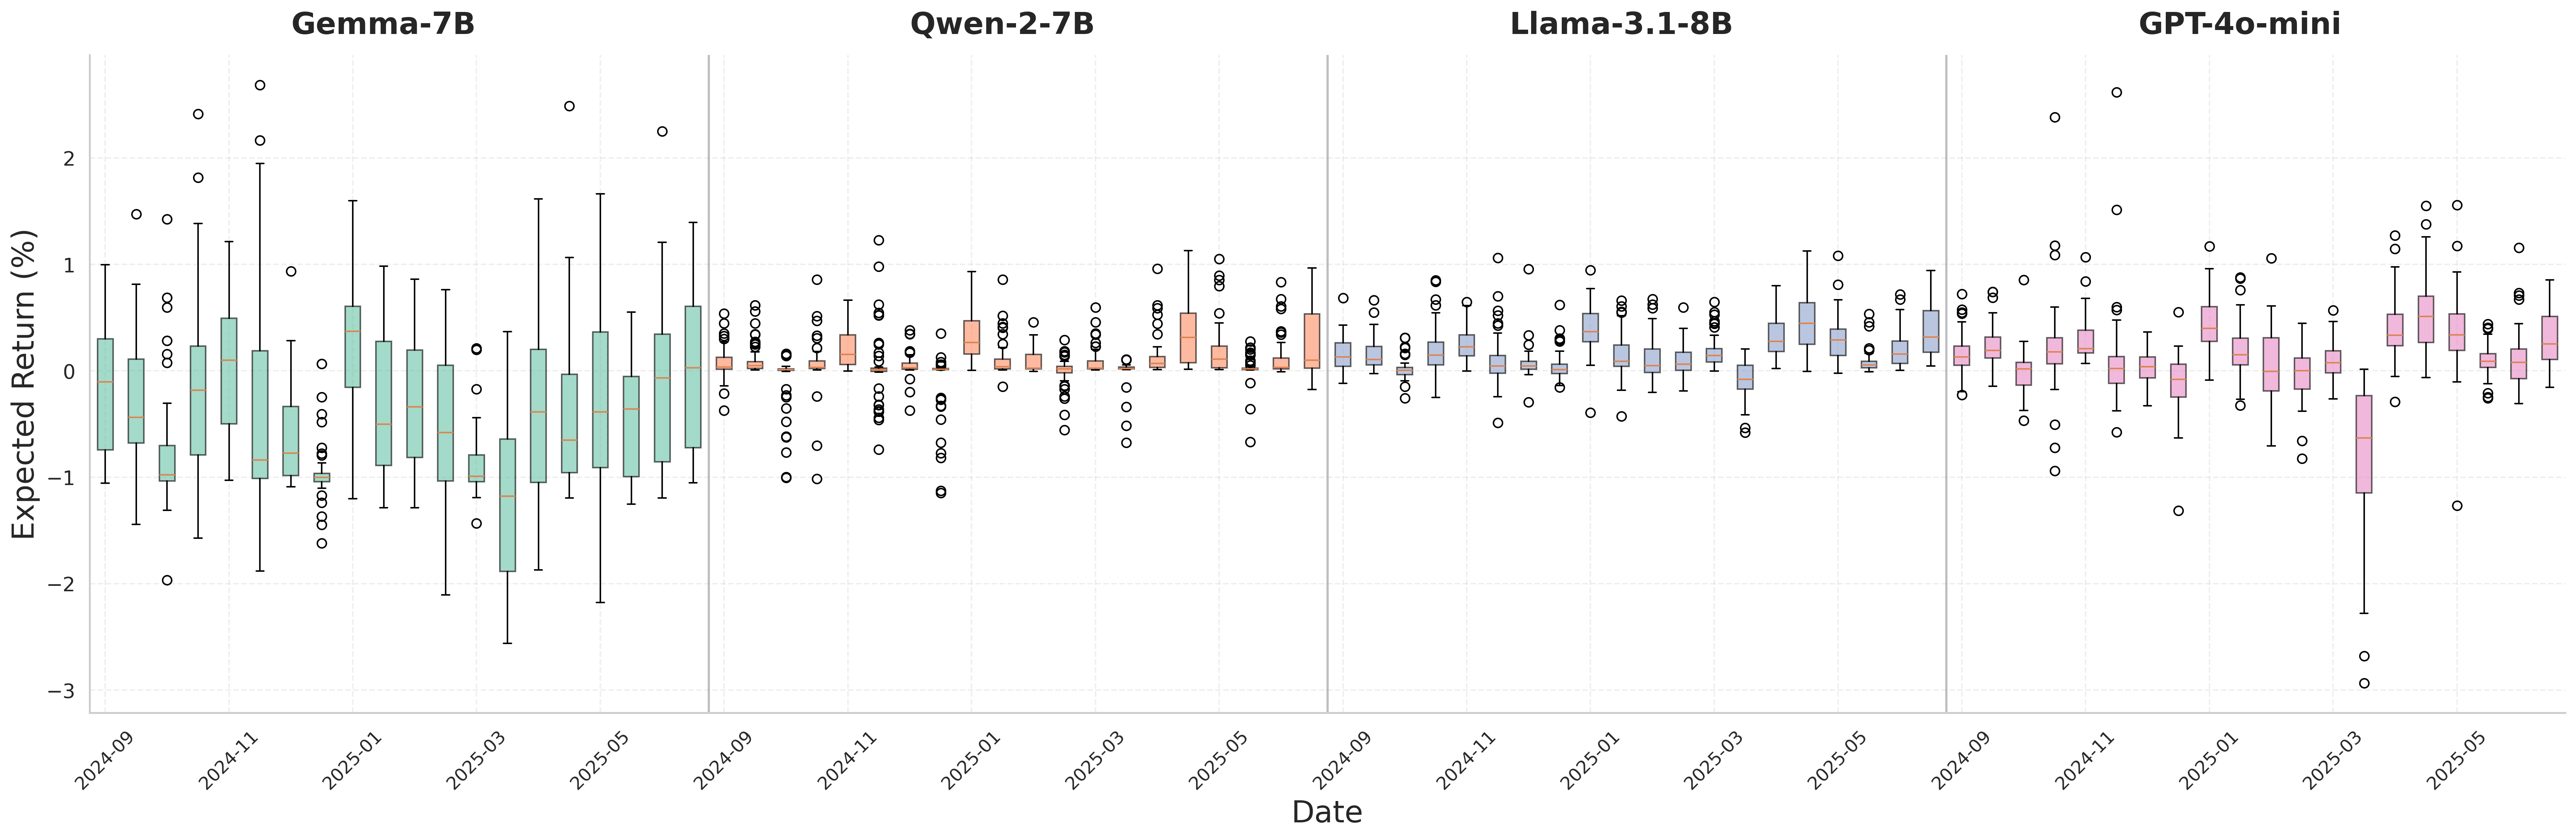
\includegraphics[width=1.0\textwidth]{figure/views_boxplot_4.png} 
    \caption{
    \textbf{LLM-generated Views Over Time at Rebalancing Intervals.} The figure visualizes the distribution of all generated return forecasts for each LLM at every rebalancing interval. 
    }
    \label{fig:boxplot} 
\end{figure}

The visual analysis highlights observable differences in the distributional patterns of each model's forecasts. These differences are consistent with recent findings that LLMs are not neutral decision-makers but possess distinct, model-specific biases \cite{lee2025your}. 
\textbf{\texttt{Gemma}} shows a relatively wider interquartile range compared to other models, indicating a higher degree of dispersion in its predicted returns. Additionally, its median values frequently sit slightly below zero, suggesting a tendency toward more conservative or negative return forecasts during the sample period.

In comparison, \textbf{\texttt{Qwen}} and \textbf{\texttt{Llama}} exhibit more concentrated distributions. Both models tend to produce forecasts clustered slightly above zero, with narrower interquartile ranges than \textbf{\texttt{Gemma}}. \textbf{\texttt{Qwen}} displays a tight core distribution while maintaining some distinct negative outliers, whereas \textbf{\texttt{Llama}} shows a similarly compact distribution. This suggests that, for this specific dataset, these models tended to generate lower-variance forecasts with a slightly positive central tendency.

Finally, \textbf{\texttt{GPT}} demonstrates variability in its dispersion over time. While often similar to the concentrated profiles of \textbf{\texttt{Qwen}} and \textbf{\texttt{Llama}}, it shows periods of increased variance, such as around March 2025, where the distribution widens and extends into negative territory.

Overall, these results indicate that even when prompted with the same instructions, different LLMs yield varying distributions of expected returns. \textbf{\texttt{Qwen}} and \textbf{\texttt{Llama}} provided more stable and slightly positive signals compared to the wider dispersion observed in \textbf{\texttt{Gemma}}. These distributional characteristics—specifically the lower variance and positive drift—likely contributed to the differences in portfolio allocation and subsequent performance discussed in the previous section.

Table~\ref{tab:view_statistics} provides the summary statistics for the entire population of raw views generated by each LLM throughout the test period. These statistics further illustrate the distributional differences suggested by the preceding visual analysis. For instance, \textbf{\texttt{Llama}} exhibits the highest mean return together with the largest standard deviation and the widest min-max range. In contrast, \textbf{\texttt{Qwen}} has the lowest standard deviation, while \textbf{\texttt{Gemma}} shows a negative mean during the sample period. Taken together, these summary statistics are broadly consistent with the differences in center and dispersion discussed above and may help explain the differences in portfolio behavior and performance.

\begin{table}[h!]
    \centering
    \caption{Summary Statistics of LLM-Generated Views}
    \label{tab:view_statistics}
    \renewcommand{\arraystretch}{1.2}
    % siunitx 설정: 숫자를 소수점 4자리로 정렬
    \sisetup{
        round-mode=places,
        round-precision=4,
        table-format=-2.4 % 부호, 정수 2자리, 소수 4자리
    }
    \small
    \setlength{\tabcolsep}{5pt}
    \begin{tabular}{l S S S S}
    \toprule
    \textbf{Metric} & {\textbf{\texttt{Gemma-7B}}} & {\textbf{\texttt{Qwen-2-7B}}} & {\textbf{\texttt{Llama-3.1-8B}}} & {\textbf{\texttt{GPT-4o-mini}}} \\
    \midrule
    \textbf{Count}      & \multicolumn{1}{c}{1000} & \multicolumn{1}{c}{1000} & \multicolumn{1}{c}{1000} & \multicolumn{1}{c}{1000} \\
    \textbf{Mean}       & -0.3847       & 0.1007        & 0.1786        & 0.1347        \\
    \textbf{Std}        & 0.7492        & 0.2430        & 0.2248        & 0.4171        \\
    \textbf{Min}        & -2.5617       & -1.1486       & -0.5812       & -2.9331       \\
    \textbf{25\%}       & -0.9917       & 0.0159        & 0.0290        & -0.0299       \\
    \textbf{Median}     & -0.5152       & 0.0343        & 0.1169        & 0.1295        \\
    \textbf{75\%}       & 0.1607        & 0.1519        & 0.2923        & 0.3191        \\
    \textbf{Max}        & 2.6854        & 1.2284        & 1.1264        & 2.6172        \\
    \bottomrule
    \end{tabular}
\par\small\textit{Note:} All metrics except `Count' are expressed in percentages (\%).
\end{table} % \label{tab:view_statistics}

\subsection{RQ3: Investment Styles - Confidence}

Finally, we investigate the association between the model-implied confidence and the realized prediction error. In the BLM framework, this relationship is relevant because the confidence matrix $\Omega$ acts as a weighting mechanism: views with higher volatility are effectively down-weighted during the posterior update. Figure~\ref{fig:scatter} plots the correlation between view standard deviation (x-axis) and RMSE (y-axis) for each model, superimposed with linear regression lines.

\begin{wrapfigure}{r}{0.5\textwidth}
    \centering
    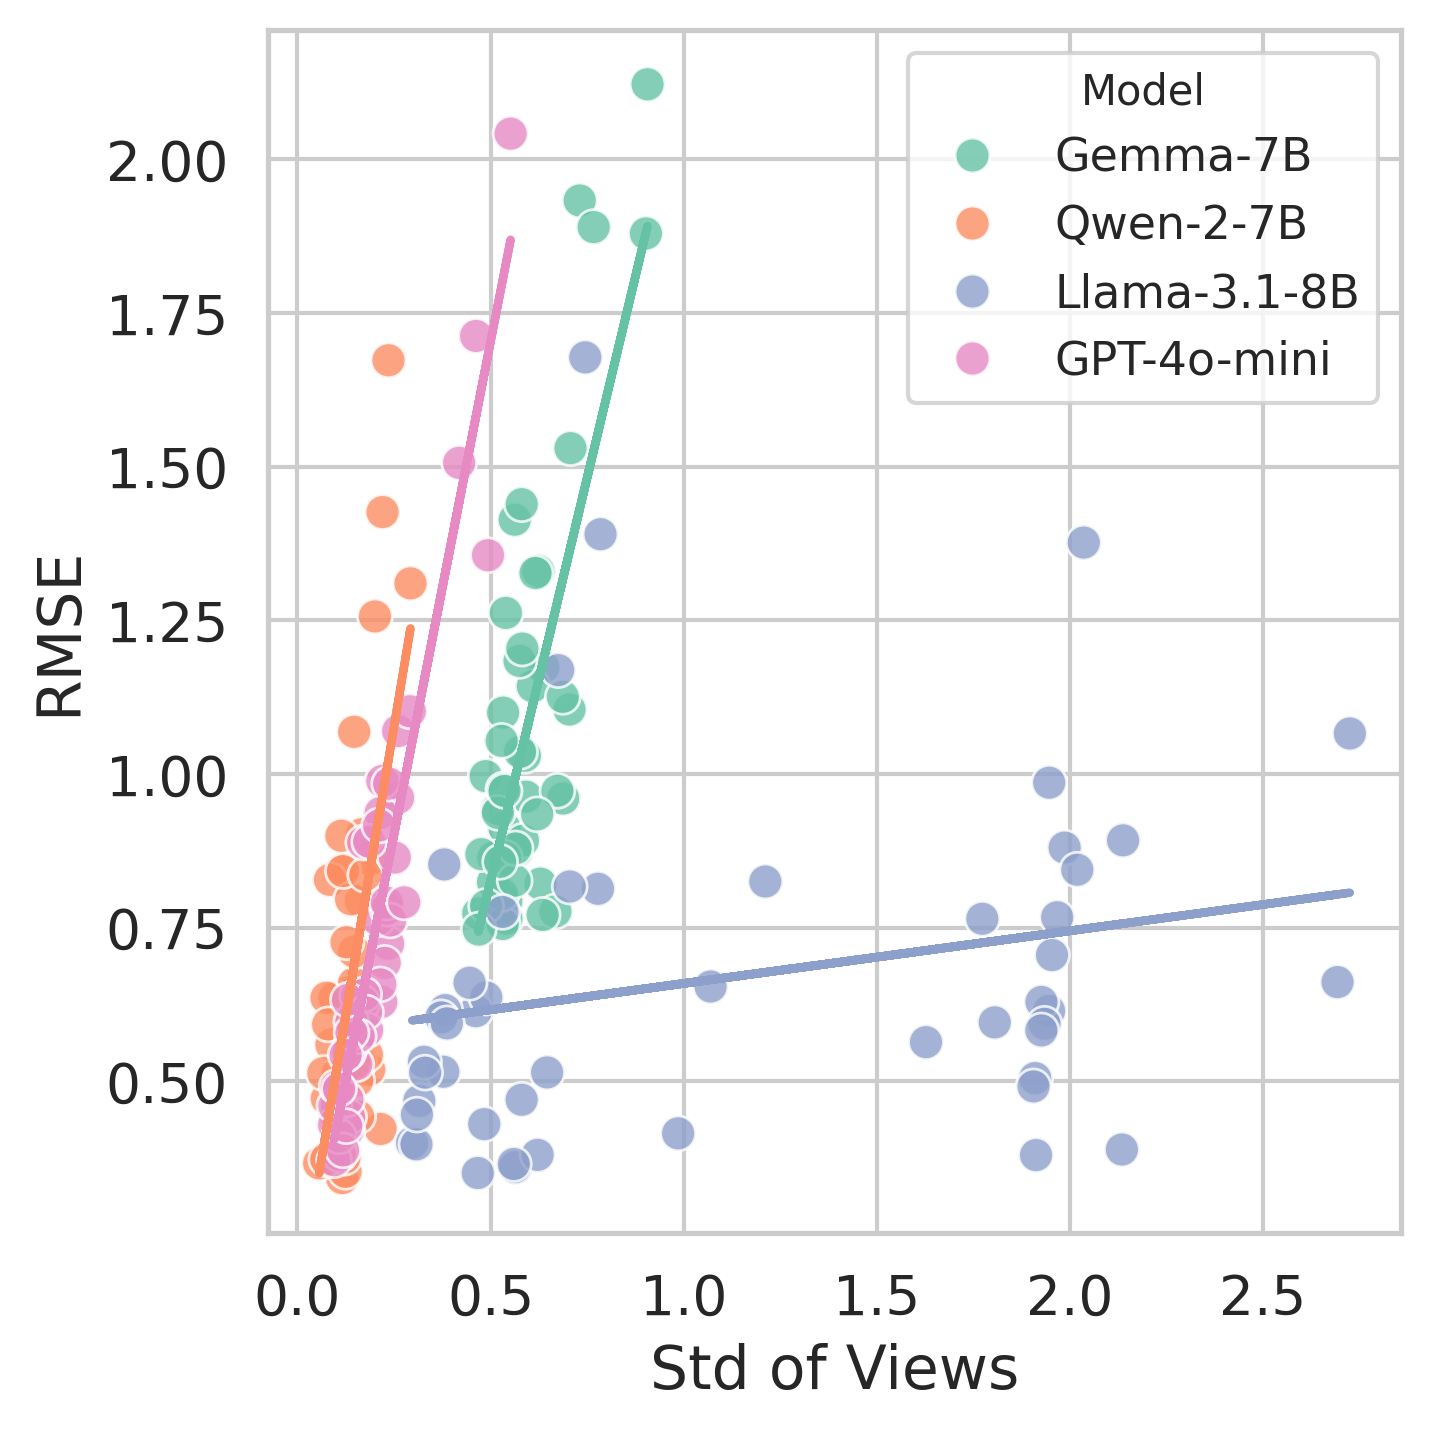
\includegraphics[width=\linewidth]{figure/scatter_4_scaled-none.png}
    \caption{\textbf{Correlation between view standard deviation and prediction error.}   }
    \label{fig:scatter}
    \vspace{-10pt} 
\end{wrapfigure}

\textbf{\texttt{Llama}} exhibits a relatively flat trajectory. The regression line has a near-zero slope ($0.086$) positioned at the lowest RMSE level among the tested models. This indicates that, in our experiment, \textbf{\texttt{Llama}}'s prediction error remained consistently low regardless of the magnitude of its estimated variance. This suggests that the model's contribution to the portfolio was driven primarily by its lower baseline error rather than the variance-based filtering mechanism.

In contrast, \textbf{\texttt{Qwen}} demonstrates the steepest positive slope ($3.751$). This positive correlation implies that instances where the model reported lower variance (higher confidence) tended to correspond with lower prediction errors. Within the BLM framework, this alignment allows the optimizer to effectively down-weight predictions that are likely to have high variance (low confidence), potentially aiding portfolio stability. This observation shares similarities with the findings in \cite{lee2025return}, which highlighted that portfolio performance is often driven by accurate predictions specifically for the assets selected in the portfolio, rather than global accuracy. 

Conversely, \textbf{\texttt{Gemma}} (slope: $2.621$) and \textbf{\texttt{GPT}} (slope: $3.204$) show distributions clustered in regions of higher overall RMSE compared to \textbf{\texttt{Llama}} and \textbf{\texttt{Qwen}}. 
While they also display positive slopes, indicating some correspondence between uncertainty and error, their generally higher prediction errors suggest that the variance filter alone was insufficient to fully mitigate the impact of inaccurate views in this specific setting.

In summary, we observe distinct patterns in how the models' uncertainty estimates relate to their accuracy. \textbf{\texttt{Llama}} is characterized by a consistently lower error profile, whereas \textbf{\texttt{Qwen}} shows a stronger alignment between uncertainty and error magnitude. These results suggest that the efficacy of LLM-based views in a Bayesian framework may depend on either maintaining a low baseline error or successfully calibrating uncertainty estimates to realized risk.